\newpage
\section{Aufgabe 1: 2D Lennard-Jones-Fluid}
\label{sec:auf1}

\subsection{Python}

In der \textit{python}-Datei "moldyn.py" ist der Code für den Verlet-Algorithmus.\\
In dieser Datei findet sowohl eine rudimentäre Simulation mittels matplotlib.pyplot statt, sowie die Datenspeicherung der zu berechnenden Größen.
\newline\\
Gemäß des Aufgabenteils a), der Initialisierung, wurde die Teilchenmatrix aufgebaut und jedem Teilchen wurde eine Anfangsgeschwindigkeit zugeordnet, die in der Summe 0 ist.
Die Anfangsgeschwindigkeit ist gemäß der Formel
\begin{equation}
    \frac{1}{2}mv^2 = k_BT \quad \text{mit} \quad m = 1
\end{equation}
umskalierbar mit der Temperatur.\\
Im Programmcode wurde der korrekte Wert für $k_B$ genommen, er kann aber auch auf andere Werte gesetzt werden, da unsere Masse überproportional groß für diese Formel ist.
\newpage
Für Aufgabenteil b) sollten das System bei der Temperatur $T(0) = 1$ starten und die Schwerpunktgeschwindigkeit, die Temperatur, die potentielle und kinetische Energie als Funktion der Zeit aufgetragen werden.\\
Die geforderte Äquilibrierung konnte nicht erreicht werden, da das System früher oder später immer explodiert.
Die Erklärung hierzu ist wie folgt:\\
Der Zeitschritt $h=0.01$ ist bei höheren Geschwindigkeiten der Teilchen ein Hindernis.
Denn da unsere Schrittweite gebunden ist an die Position der Teilchen, werden sie bei höheren Geschwindigkeiten zu nah an andere Teilchen gesetzt, was im Lennard-Jones-Potential zu sehr hohen Abstoßkräften führt.
Dadurch besitzen früher oder später alle Teilchen unrealistisch hohe Geschwindigkeiten.
Natürlich wurde bedacht die Schrittweite niedriger zu wählen, jedoch entspricht die Absetzung auf $h=0.001$ eine Verzehnfachung der Rechenzeit.
Eine Schrittweite $>$ 0 führt somit bei $t=\inf$ immer zu einer Explosion der Geschwindigkeiten.\\
\newline
Wir haben im folgenden drei verschiedene Systemparameter gewählt und jeweils die erforderlichen Graphen erstellt.
\subsubsection{Kleines Zeitintervall}
Für die folgenden Graphen wurden die Parameter so gewählt:
\begin{itemize}
    \item $T = 1$
    \item $k_B = 1.38\cdot10^{-23}$
    \item $t = 20$
    \item $h = 0.01$
\end{itemize}
Hierbei sei gesagt, dass diese Parameter nicht garantieren, dass das System in diesem Zeitraum nicht explodiert.
Die folgenden Graphen wurden jedoch für ein stabil gebliebenes System aufgezeichnet.
\newpage
Die Schwerpunktgeschwindigkeit ist in \autoref{fig:swp} abgebildet.
\begin{figure}[H]
    \centering
    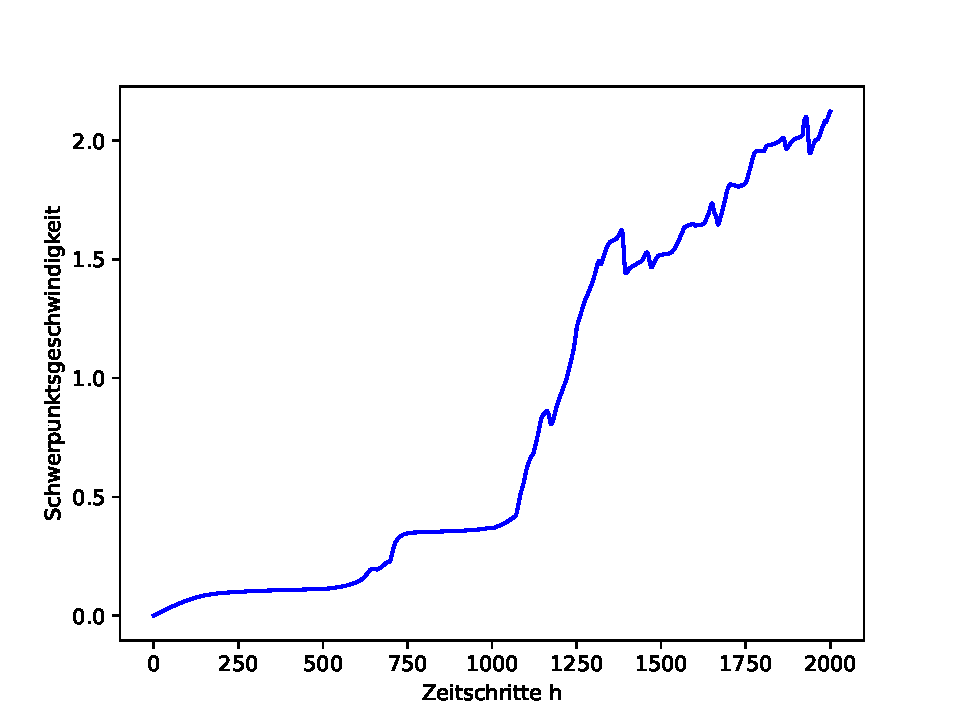
\includegraphics[scale=0.5]{MolDyn/Small Boy/swp_velocity.pdf}
    \caption{In dieser Abbildung ist der zeitliche Verlauf der Schwerpunktgeschwindigkeit aufgetragen.}
    \label{fig:swp}
\end{figure}
Die Temperatur ist in \autoref{fig:temp} abgebildet.
\begin{figure}[H]
    \centering
    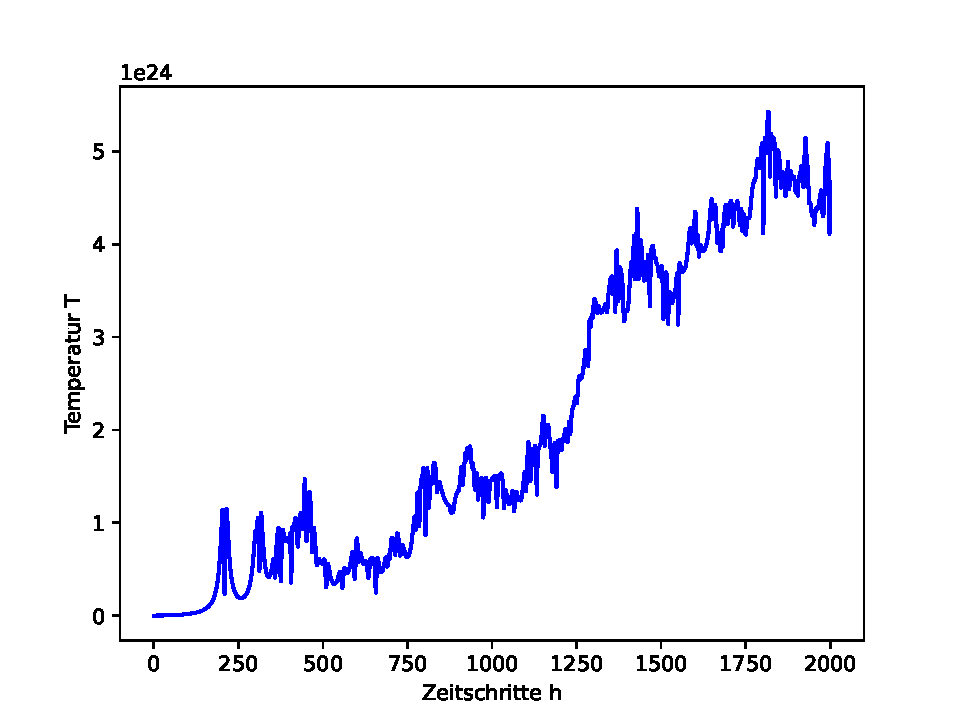
\includegraphics[scale=0.5]{MolDyn/Small Boy/temperature.pdf}
    \caption{In dieser Abbildung ist der zeitliche Verlauf der Temperatur aufgetragen.}
    \label{fig:temp}
\end{figure}
\newpage
Die potentielle Energie ist in \autoref{fig:pot} abgebildet.
\begin{figure}[H]
    \centering
    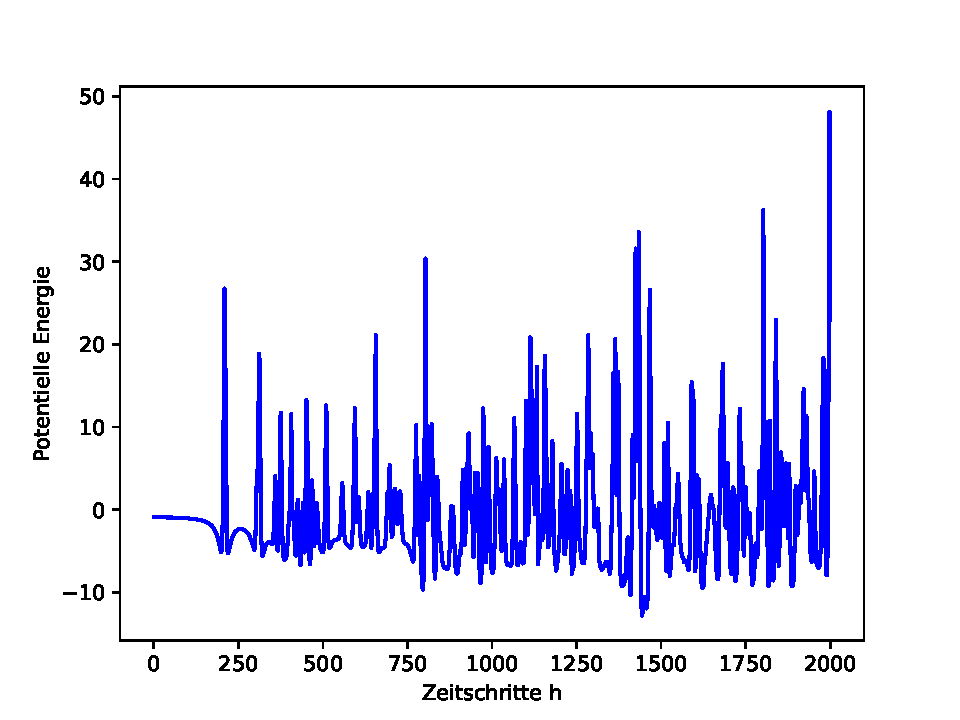
\includegraphics[scale=0.5]{MolDyn/Small Boy/potential_energy.pdf}
    \caption{In dieser Abbildung ist der zeitliche Verlauf der potentiellen Energie aufgetragen.}
    \label{fig:pot}
\end{figure}
Die kinetische Energie ist in \autoref{fig:kin} abgebildet.
\begin{figure}[H]
    \centering
    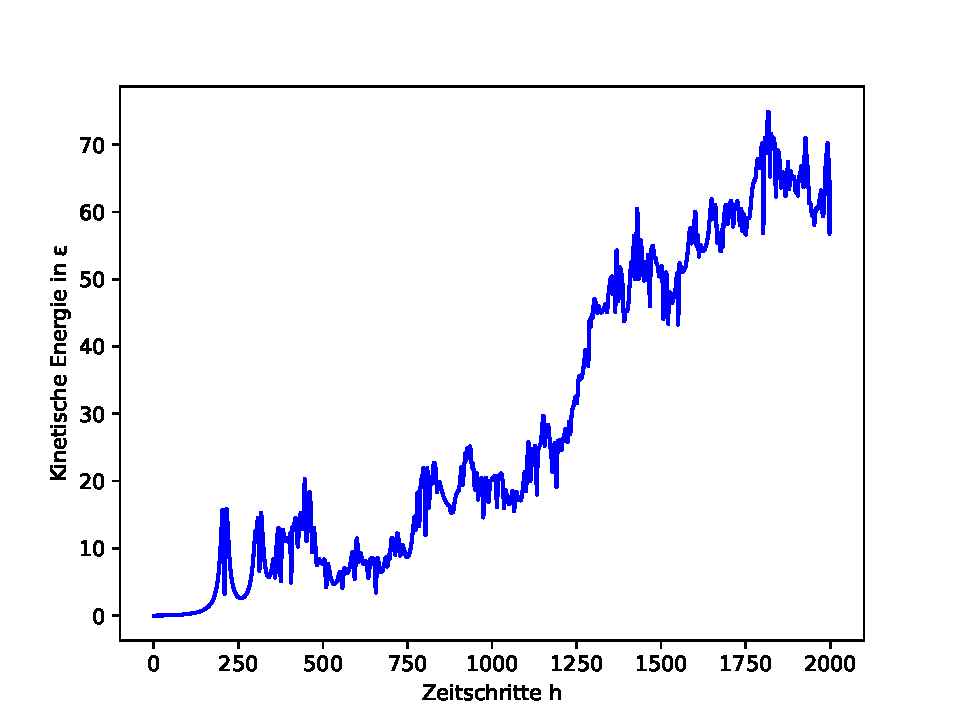
\includegraphics[scale=0.5]{MolDyn/Small Boy/kinetic_energy.pdf}
    \caption{In dieser Abbildung ist der zeitliche Verlauf der kinetischen Energie aufgetragen.}
    \label{fig:kin}
\end{figure}
\newpage
\subsubsection{Mittleres Zeitintervall}
Für die folgenden Graphen wurden die Parameter so gewählt:
\begin{itemize}
    \item $T = 1$
    \item $k_B = 1.38\cdot10^{-23}$
    \item $t = 100$
    \item $h = 0.01$
\end{itemize}
Es passiert unweigerlich eine Explosion in den Daten, die deutlich in den Abbildungen zu sehen ist.
Hierbei handelt es sich offensichtlich nicht um die Äquilibrierung, sondern die vorher besprochene Folge des $h\neq0$.
\newpage
Die Schwerpunktgeschwindigkeit ist in \autoref{fig:swp1} abgebildet.
\begin{figure}[H]
    \centering
    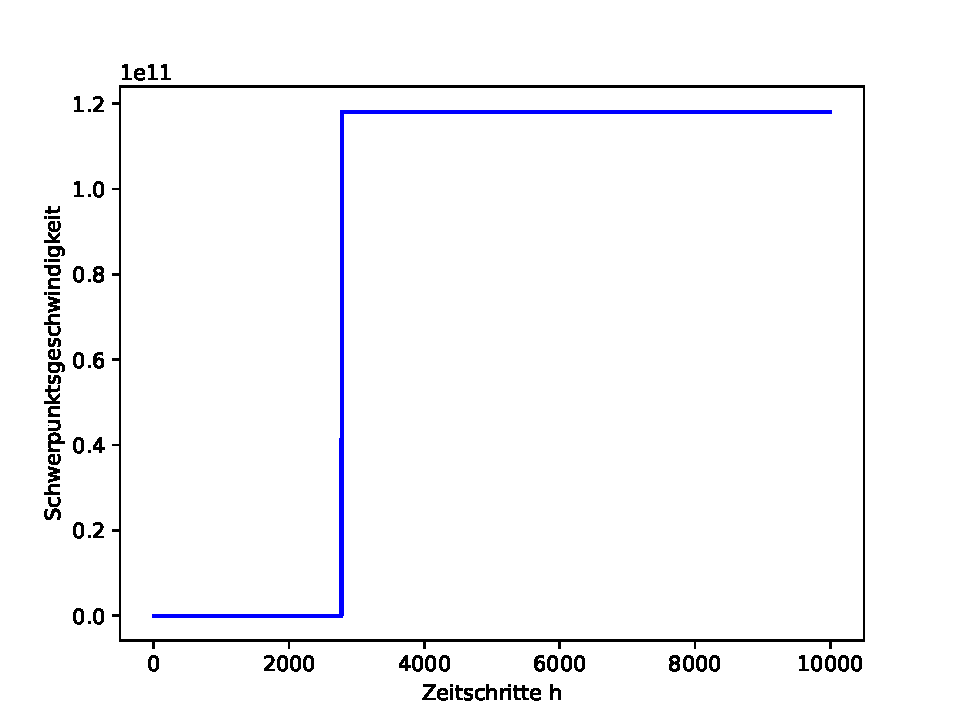
\includegraphics[scale=0.5]{MolDyn/Medium Boy/swp_velocity.pdf}
    \caption{In dieser Abbildung ist der zeitliche Verlauf der Schwerpunktgeschwindigkeit aufgetragen.}
    \label{fig:swp1}
\end{figure}
Die Temperatur ist in \autoref{fig:temp1} abgebildet.
\begin{figure}[H]
    \centering
    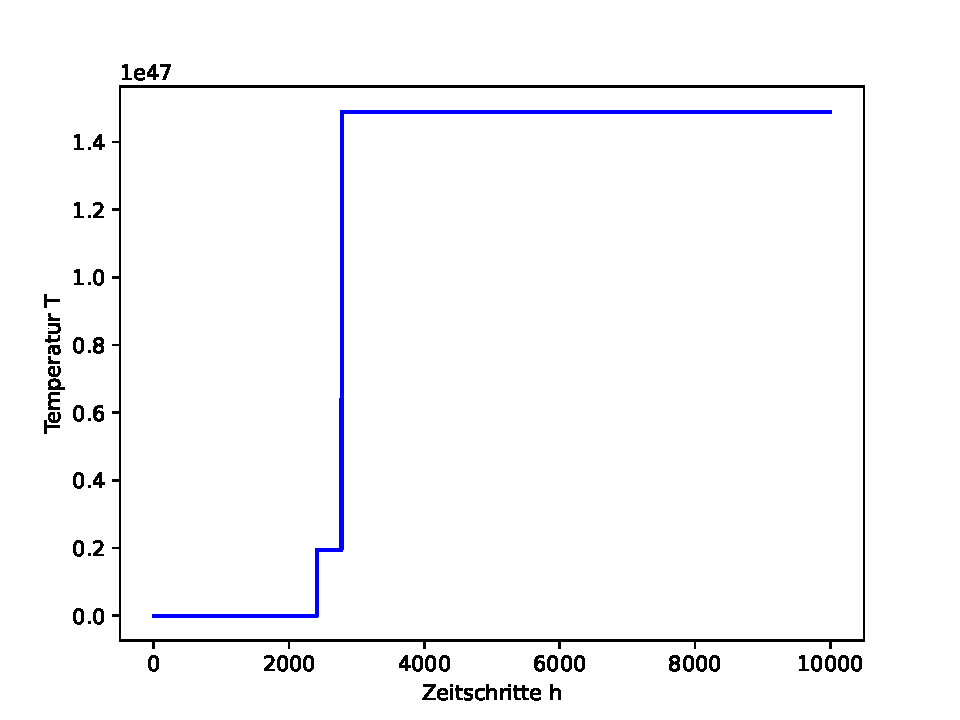
\includegraphics[scale=0.5]{MolDyn/Medium Boy/temperature.pdf}
    \caption{In dieser Abbildung ist der zeitliche Verlauf der Temperatur aufgetragen.}
    \label{fig:temp1}
\end{figure}
\newpage
Die potentielle Energie ist in \autoref{fig:pot1} abgebildet.
Es sind im Plot nicht die vollen Zeitschritte dargestellt, da ab einer bestimmten Geschwindigkeit von zwei Teilchen, deren Abstand so gering wird, dass dieser $r^6$ oder $r^{12}$ im Code als Null angesehen wird.
Da es sich dann um eine Teilung durch Null handelt, werden diese Werte nicht im Plot berücksichtigt.
\begin{figure}[H]
    \centering
    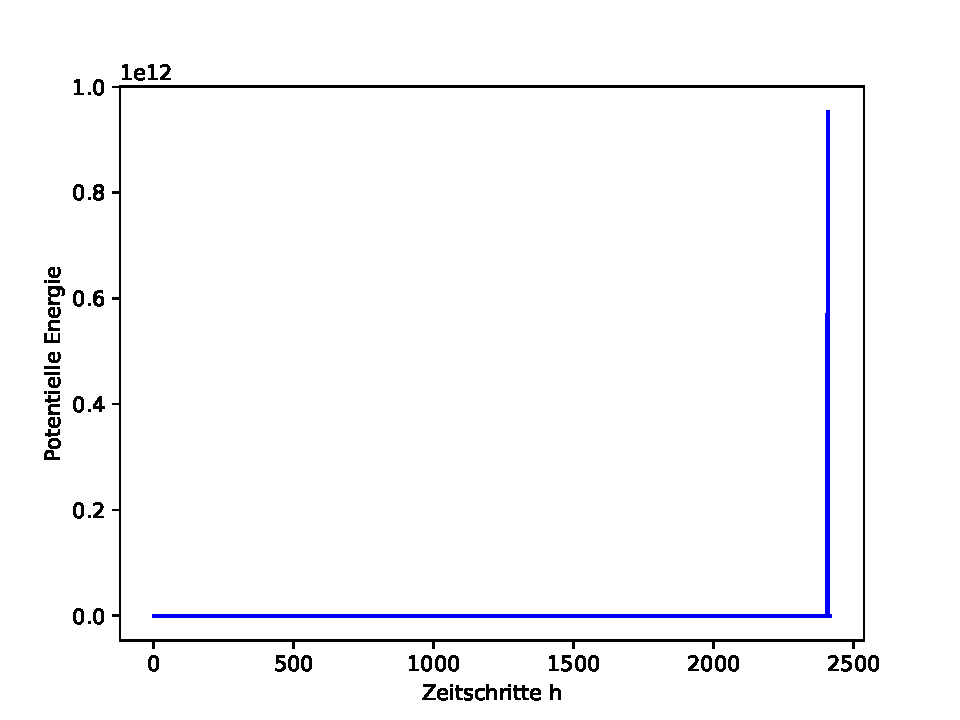
\includegraphics[scale=0.5]{MolDyn/Medium Boy/potential_energy.pdf}
    \caption{In dieser Abbildung ist der zeitliche Verlauf der potentiellen Energie aufgetragen.}
    \label{fig:pot1}
\end{figure}
Die kinetische Energie ist in \autoref{fig:kin1} abgebildet.
\begin{figure}[H]
    \centering
    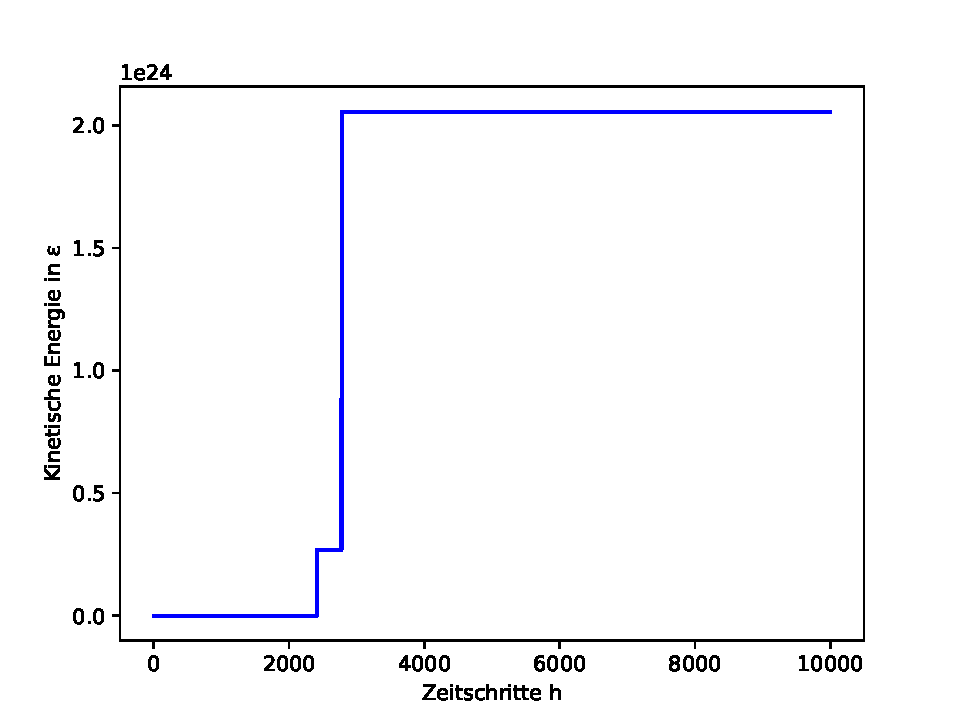
\includegraphics[scale=0.5]{MolDyn/Medium Boy/kinetic_energy.pdf}
    \caption{In dieser Abbildung ist der zeitliche Verlauf der kinetischen Energie aufgetragen.}
    \label{fig:kin1}
\end{figure}
\newpage
\subsubsection{Großes Zeitintervall}
Für die folgenden Graphen wurden die Parameter so gewählt:
\begin{itemize}
    \item $T = 100$
    \item $k_B = 1$
    \item $t = 5$
    \item $h = 0.0001$
\end{itemize}
Wie zu erkennen ist, wurde die Schrittweite um zwei Größenordnungen verkleinert, dafür jedoch nur ein Zeitintervall von 5 simuliert.
Die Temperatur und Boltzmannkonstante wurde erhöht, damit sich die Teilchen in dieser Zeitspanne signifikant bewegen.\\
In den Abbildungen \ref{fig:kin2}, \ref{fig:temp2} und \ref{fig:swp2} sind deutliche Plateaus zu erkennen, die sehr wahrscheinlich auch Äquilibrierungs-Potential hätten.
Aber wie bereits erwähnt, ist die Schrittweite auch hier für das Anwachsen der Geschwindigkeit verantwortlich.\\
Diese Anzahl von Schritten resultierte in einer $1\frac{1}{2}$-stündigen Rechenzeit.
\newpage
Die Schwerpunktgeschwindigkeit ist in \autoref{fig:swp2} abgebildet.
\begin{figure}[H]
    \centering
    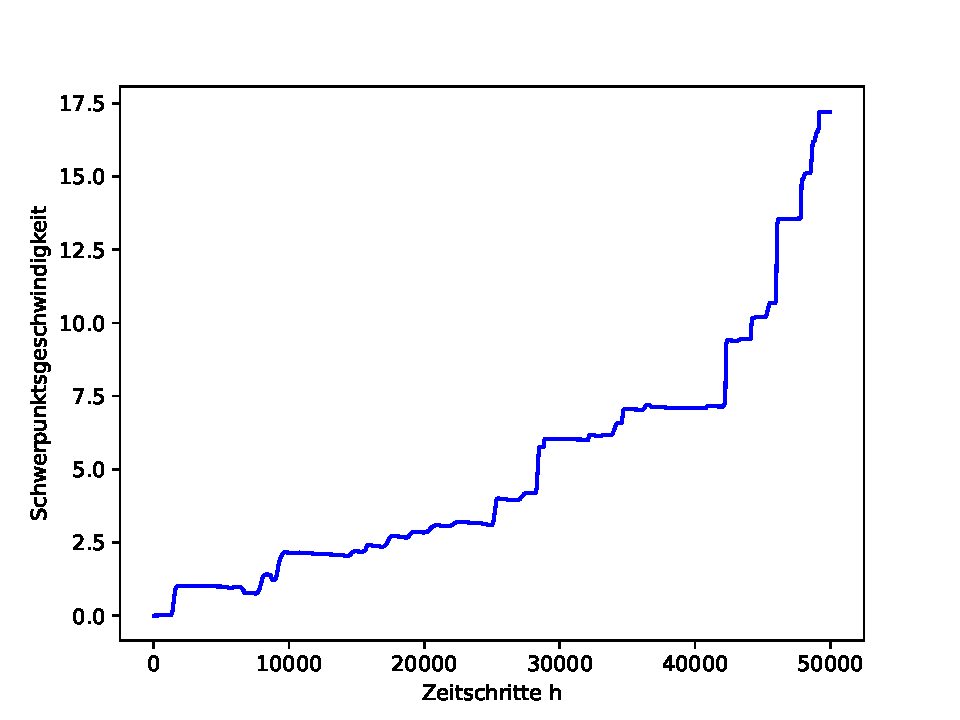
\includegraphics[scale=0.5]{MolDyn/Big Boy/swp_velocity.pdf}
    \caption{In dieser Abbildung ist der zeitliche Verlauf der Schwerpunktgeschwindigkeit aufgetragen.}
    \label{fig:swp2}
\end{figure}
Die Temperatur ist in \autoref{fig:temp2} abgebildet.
\begin{figure}[H]
    \centering
    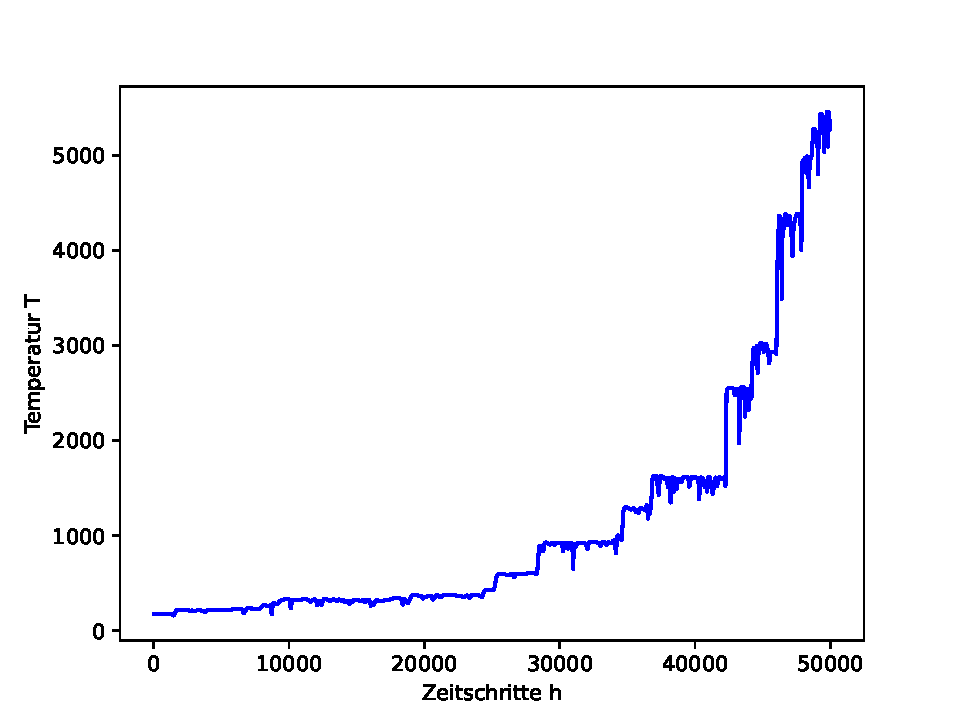
\includegraphics[scale=0.5]{MolDyn/Big Boy/temperature.pdf}
    \caption{In dieser Abbildung ist der zeitliche Verlauf der Temperatur aufgetragen.}
    \label{fig:temp2}
\end{figure}
\newpage
Die potentielle Energie ist in \autoref{fig:pot2} abgebildet.
\begin{figure}[H]
    \centering
    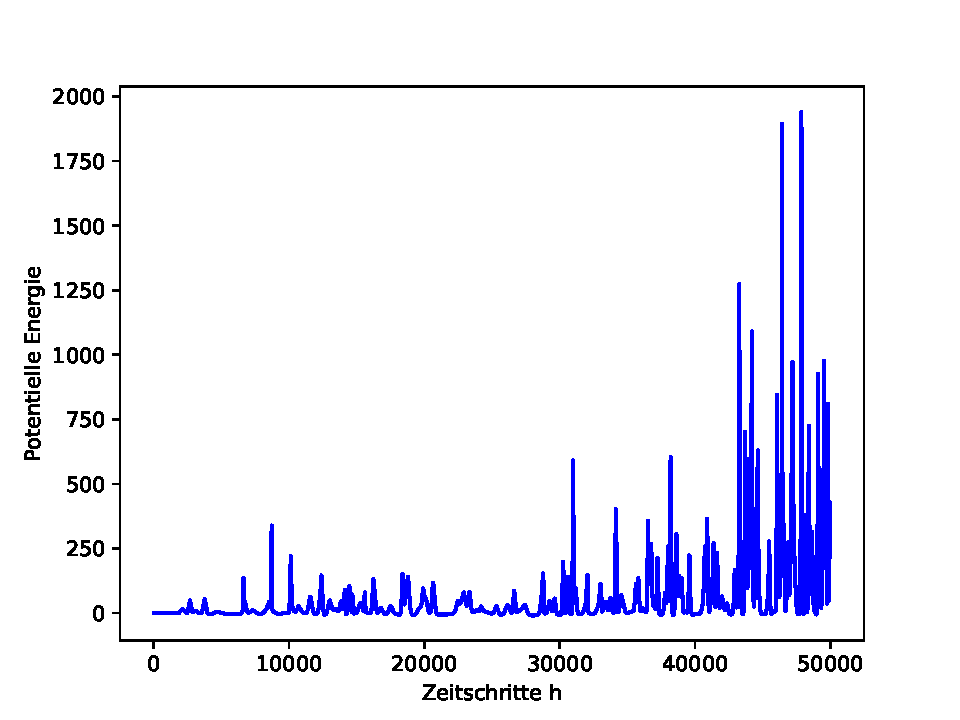
\includegraphics[scale=0.5]{MolDyn/Big Boy/potential_energy.pdf}
    \caption{In dieser Abbildung ist der zeitliche Verlauf der potentiellen Energie aufgetragen.}
    \label{fig:pot2}
\end{figure}
Die kinetische Energie ist in \autoref{fig:kin2} abgebildet.
\begin{figure}[H]
    \centering
    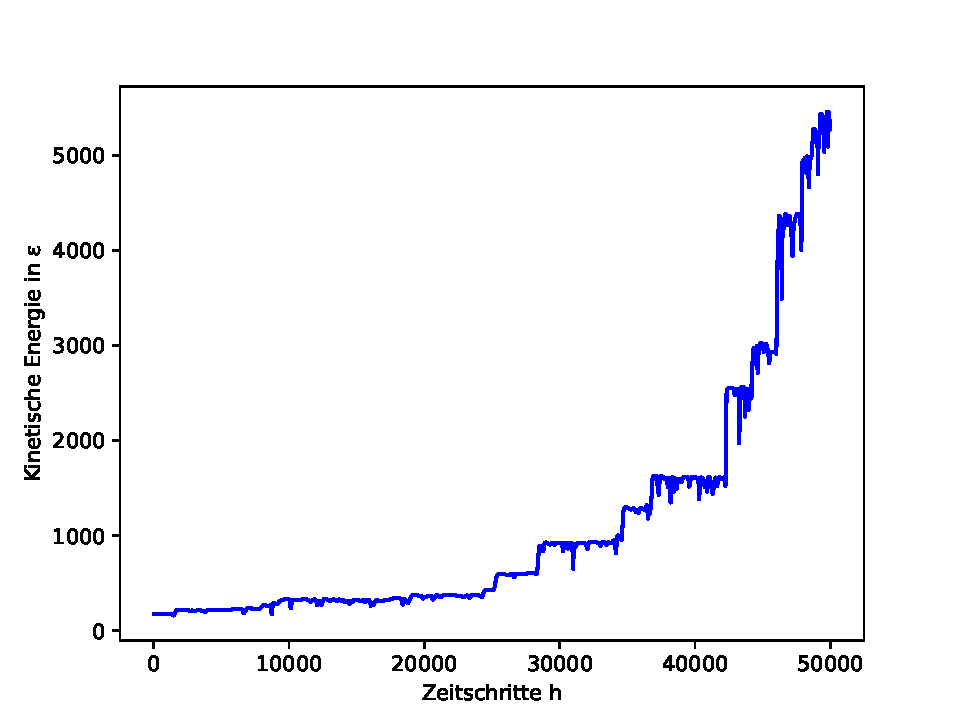
\includegraphics[scale=0.5]{MolDyn/Big Boy/kinetic_energy.pdf}
    \caption{In dieser Abbildung ist der zeitliche Verlauf der kinetischen Energie aufgetragen.}
    \label{fig:kin2}
\end{figure}
Zusammenfassend ist anzumerken, dass sich aufgrund der fehlenden Äquilibrierung keine korrekte Paarkorrelationsfunktion darstellen lässt.
\newpage

\subsection{C++}